\chapter{Aprendizaje Automático y AutoML}\label{chap:1}

En este primer capítulo, se aborda el marco teórico de la tesis, el cual se enfoca en diferentes temas clave dentro del campo de la inteligencia artificial y la minería de datos. En particular, se discute el aprendizaje automático, el descubrimiento de conocimiento en bases de datos, la minería de datos y la clasificación. Además, se introduce el concepto de AutoML, como herramienta para automatizar el proceso de pre-procesado y optimización de hiperparámetros en la implementación de técnicas de aprendizaje automático. Por último, se destaca la importancia de la plataforma KNIME como una herramienta útil para la implementación de técnicas de AutoML y análisis de datos.

\section{Proceso de descubrimiento de conocimiento en bases de datos}\label{kdd}
La Extracción de Conocimiento en Bases de Datos (\textit{Knwodlege Discovery from Databases}, o \textit{KDD} por sus siglas en inglés) se define como: “el proceso no trivial de identificar patrones válidos, novedosos, potencialmente útiles y, en última instancia, comprensibles a partir de los datos” \citep{orallo2004}. Este proceso está compuesto por una serie de etapas o fases, descritas a continuación:
\begin{itemize}
	\item Integración y recopilación: Es donde se decide qué datos serán utilizados en el proceso de KDD. Esto implica la selección de fuentes de datos relevantes y la adquisición de los conjuntos de datos necesarios.  Como parte del desarrollo de esta fase, es necesario diseñar o conocer el modo en que se van a organizar e integrar los datos; con el fin de eliminar redundancias e inconsistencias.
	\item Selección, limpieza y transformación: Se seleccionan los datos más relevantes y que aporten mejor información, garantizando que tengan la mejor calidad posible, logrando obtener la vista minable con los datos listos para la aplicación del algoritmo.
	\item Algoritmos de Minería de datos: En esta etapa central del proceso, se aplican algoritmos de minería de datos para identificar patrones, tendencias o estructuras en los datos. Esto puede incluir la clasificación, la segmentación, la regresión y otras técnicas de análisis.
	\item Evaluación e Interpretación: El objetivo de esta etapa es medir la calidad de los modelos obtenidos, utilizando diferentes métricas de calidad, las cuales dependen de las técnicas de minería de datos que se utilicen. La interpretación de los resultados se apoya en el uso de técnicas de visualización y de representación, con el fin de comprender mejor el conocimiento aportado. 
	\item Difusión y uso: En esta etapa, se integra el conocimiento obtenido de la comprensión del negocio, con el conocimiento de los modelos de minería de datos usado en la toma de decisiones de los especialistas. La monitorización de los patrones debe realizarse, pues en ocasiones resulta necesaria la reevaluación del modelo, su reentrenamiento o incluso su reconstrucción total.
\end{itemize}

En el contexto de la creciente acumulación de datos en instituciones que han digitalizado sus registros históricos en bases de datos, la extracción de información valiosa a través de patrones ocultos se convierte en un desafío crucial. La magnitud de esta información a menudo supera las capacidades de análisis de los expertos, lo que hace imperativo recurrir a técnicas automatizadas. Por lo tanto, la Minería de Datos emerge como una necesidad vital dentro del proceso KDD, ya que permite desentrañar conocimiento significativo y no evidente en estos vastos conjuntos de datos.

\subsection{Minería de Datos}
Acorde a \citep{orallo2004}, la minería de datos es definida como el proceso de extraer conocimiento útil y comprensible, previamente desconocido, desde grandes cantidades de datos almacenados en distintos formatos. \\
El conocimiento extraído se puede presentar en forma de relaciones, patrones o reglas inferidas de los datos, o en forma de descripción un poco más concisa. Estos constituyen un modelo de datos analizados. Estos modelos, o tareas, se categorizan en predictivas y descriptivas \citep{orallo2004}. \\
En las tareas predictivas, los ejemplos están etiquetados y se emplean para estimar valores futuros o desconocidos de variables de interés. En este entorno se encuentra el aprendizaje supervisado. En cambio, las tareas descriptivas son empleadas en el descubrimiento de propiedades de los datos examinados donde los ejemplos no se encuentran etiquetados. Aquí se pone de manifiesto el aprendizaje no supervisado. En \citep{orallo2004} se describen las tareas de minería de datos de la siguiente manera:
\begin{itemize}
	\item Clasificación: La clasificación se encarga de examinar las características de un registro u objeto, y de esta forma asignarle una clase predefinida. Estas clases son valores discretos. Para ello, se tiene que construir un modelo a partir de datos previamente clasificados. Como variantes a la clasificación, existe el aprendizaje de “rankings”, aprendizaje de preferencias y el aprendizaje de probabilidad, entre otros. 
	\item Regresión: A diferencia de la clasificación, el valor a predecir es numérico. Consiste en aprender una función real que calcula un valor para un atributo real. Su objetivo es minimizar el error entre el valor predicho y el valor real.
	\item  Correlaciones: Son empleadas para examinar el grado de similitud de los valores de dos variables numéricas. Se basa en el cálculo de correlación de variables numéricas usando la estadística. Este método trata de determinar si el comportamiento de dos variables numéricas está relacionado.
	\item Reglas de asociación: Son situaciones o características que ocurren en un mismo instante de tiempo. Pueden ser relaciones causales o casuales. Representan patrones de comportamiento entre los datos en función de la aparición conjunta de valores de dos o más atributos. Las medidas habituales propuestas en \citep{Agrawal1519}	para establecer la idoneidad y el interés de una regla de asociación son la confianza y el soporte.
	\item	Agrupamiento (Clustering): Para realizar esta tarea se parte de datos sin clasificar, teniendo como objetivo segmentar un grupo de datos diversos en subgrupos. Los miembros de cada grupo (clúster, por su definición en inglés) deben tener mucho en común entre sí y, a su vez, diferenciarse del resto de elementos de otros grupos. Dado que la clasificación de estos grupos no se conoce previamente, es el minero el encargado de darles un significado.
\end{itemize}

La minería de datos, como etapa inicial en la exploración y extracción de conocimiento a partir de grandes conjuntos de datos, sienta las bases para el aprendizaje automático, una disciplina de la inteligencia artificial que se centra en el desarrollo de algoritmos y modelos capaces de aprender patrones y realizar tareas de toma de decisiones basadas en datos.

\section{Aprendizaje Automático}
Uno de los campos más destacados dentro de la Inteligencia Artificial es el Machine Learning (Aprendizaje Automático), que es un enfoque que utiliza algoritmos y modelos matemáticos para permitir que los sistemas aprendan de los datos y realicen tareas específicas sin ser programados explícitamente.
Se define el Aprendizaje Automático como un conjunto de métodos que pueden detectar automáticamente patrones en los datos y luego, usar los patrones descubiertos para predecir datos futuros, o para realizar otros tipos de toma de decisiones bajo incertidumbre \citep{murphy2012machine}. Es decir, es el proceso en el que las computadoras descubren cómo hacer cosas sin estar específicamente programadas para hacerlo \citep{Praba2021}. Por lo tanto, el objetivo principal del aprendizaje automático es estudiar, diseñar y mejorar modelos matemáticos que se pueden entrenar (una vez o continuamente) con datos relacionados con el contexto (proporcionados por un entorno genérico), para inferir el futuro y tomar decisiones sin completo conocimiento de todos los elementos que influyen (factores externos) \citep{bonaccorso2017machine}. \\
Existen varios tipos de aprendizaje en Machine Learning, cada uno con sus propias técnicas y enfoques. A continuación, se presenta una breve descripción de algunos de los tipos de aprendizaje más comunes:
\begin{itemize}
	\item Aprendizaje supervisado: se refiere a cualquier proceso de aprendizaje automático que aprende una función de un tipo de entrada a un tipo de salida, utilizando datos que comprenden ejemplos que tienen valores de entrada y salida. Dos ejemplos típicos de aprendizaje supervisado son el aprendizaje de clasificación y la regresión \citep{sammut2011encyclopedia}. 
	\item Aprendizaje no supervisado: se refiere a cualquier proceso de aprendizaje automático que busca aprender la estructura en ausencia de un resultado identificado o retroalimentación. Tres ejemplos típicos de aprendizaje no supervisado son agrupamiento, reglas de asociación y mapas de autoorganización \citep{sammut2011encyclopedia}. 
	\item Aprendizaje por refuerzo: describe una gran clase de problemas de aprendizaje, característicos de los agentes autónomos que interactúan en un entorno: problemas de toma de decisiones secuenciales con recompensa retrasada. Los algoritmos de aprendizaje por refuerzo buscan aprender una política (mapeo de estados a acciones) que maximice la recompensa recibida a lo largo del tiempo. A diferencia de los problemas de aprendizaje supervisado, en los problemas de aprendizaje por refuerzo no hay etiquetas de ejemplo de comportamiento correcto e incorrecto. Sin embargo, a diferencia de los problemas de aprendizaje no supervisados, se puede percibir una señal de recompensa \citep{sammut2011encyclopedia}.
	\item Aprendizaje semisupervisado: es una clase de técnicas de aprendizaje automático que hacen uso de ejemplos etiquetados y no etiquetados para aprender un modelo. Los ejemplos etiquetados se usan para aprender modelos de clase y los ejemplos no etiquetados se usan para refinar los límites entre clases \citep{Han2011}.
\end{itemize}


A medida que la cantidad de datos disponibles continúa creciendo exponencialmente, y la complejidad de los modelos de Machine Learning aumenta, surge una necesidad cada vez mayor de contar con herramientas y técnicas que permitan a los usuarios automatizar el proceso de construcción de modelos. Es aquí donde entra en juego el Aprendizaje Automático Automatizado.


\begin{comment}
En particular, una de las técnicas centrales del aprendizaje supervisado es la clasificación, mencionada anteriormente como una de las tareas de la minería de datos, que permite a los algoritmos asignar etiquetas a datos y reconocer patrones subyacentes. Esta habilidad de clasificar datos en categorías predefinidas se traduce en una amplia gama de aplicaciones, lo que demuestra su versatilidad en la resolución de problemas del mundo real.
\end{comment}

%Texto... Es una buena práctica culminar (o iniciar) cada epígrafe con una referencia al que sigue (o precede) para dar fluidez a su lectura y no se vea como un \emph{copia y pega} sin ninguna relación.
         

\section{\textit{AutoML}}

El campo del Aprendizaje Automático Automatizado (AutoML), tiene como objetivo tomar decisiones de una manera automatizada, objetiva y basada en datos: el usuario simplemente proporciona datos y el sistema AutoML determina automáticamente el enfoque que funciona mejor para esta aplicación en particular \citep{hutter2019automated}. \\
AutoML (Automated Machine Learning) es una técnica que tiene como objetivo automatizar todo o parte del proceso de Machine Learning, incluyendo la selección de algoritmos, la optimización de hiperparámetros, la selección de características y la evaluación del rendimiento del modelo \citep{he2021automl}, \citep{tuggener2019automated}. La relación entre AutoML y Machine Learning es que AutoML es una técnica que se utiliza para automatizar el proceso de Machine Learning, por tanto se utiliza para automatizar todo o parte del proceso de selección del mejor modelo de Machine Learning, para un conjunto de datos dado. La automatización del proceso de Machine Learning proporciona una solución eficiente y escalable para el análisis de grandes conjuntos de datos, lo que puede resultar en un ahorro significativo de tiempo y recursos para los profesionales de ciencia de datos e investigadores. \\ 
Tras un análisis del estado del arte acerca del proceso de AutoML \citep{tuggener2019automated}, \citep{waring2020automated}, \citep{hutter2019automated}, \citep{he2021automl}, se pueden presentar como tareas principales las siguientes:
\begin{itemize}
	\item Selección de características: Esta tarea consiste en identificar las variables más relevantes para el problema de aprendizaje automático. 
	\item Pre-procesamiento de datos: La calidad de los datos de entrada es un factor crítico en el rendimiento de los modelos de aprendizaje automático. Las técnicas de preprocesamiento de datos se utilizan para limpiar, normalizar y transformar los datos de entrada en un formato que sea adecuado para el modelo. Existen varias técnicas efectivas de preprocesamiento de datos, incluyendo la eliminación de valores atípicos, la imputación de valores faltantes, la normalización y discretización de datos.
	\item Selección de modelo: Se basa en identificar el modelo de aprendizaje automático que mejor se ajusta al problema dado.
	\item Ajuste de hiperparámetros: Los modelos de aprendizaje automático tienen varios parámetros que afectan su rendimiento, y encontrar los valores óptimos de estos parámetros es una tarea importante para mejorar el rendimiento del modelo. El estado del arte ha demostrado que existen varias técnicas para el ajuste de hiperparámetros, incluyendo la búsqueda aleatoria \citep{zoller2021benchmark} y la optimización bayesiana \citep{he2021automl}, \citep{hutter2019automated}.
	\item Evaluación del modelo: La evaluación del modelo es una tarea crítica para medir el rendimiento del modelo en datos de prueba para determinar su capacidad para generalizar. Existen varias técnicas para la evaluación del modelo, incluyendo la validación cruzada y la evaluación de curvas de aprendizaje.
	\item Interpretación del modelo: Consiste en analizar el modelo de aprendizaje automático para comprender cómo se toman las decisiones y qué variables son importantes para la predicción.
\end{itemize}

En el marco de la presente investigación, se aborda de manera exhaustiva el enfoque fundamental de AutoML, centrándonos en dos aspectos cruciales que se explorarán en los epígrafes posteriores. En particular, se explorarán con detalle el pre-procesado de datos, que se enfoca en la preparación y limpieza de conjuntos de datos, y la optimización de hiperparámetros (HPO), que se concentra en la búsqueda de configuraciones óptimas para los modelos. Estos temas esenciales constituyen la base de esta investigación y servirán como pilares para la posterior discusión y análisis de resultados en este estudio. \\
En este contexto, es relevante mencionar que se establecerá una conexión crucial entre el AutoML y una plataforma  ampliamente empleada en este contexto, como lo es KNIME, un entorno de trabajo ampliamente utilizado en la comunidad científica y empresarial para la construcción y despliegue de flujos de trabajo de análisis de datos y aprendizaje automático. 


\section{Herramienta de minería de datos KNIME}

La herramienta de datos KNIME (\textit{Konstanz Information Miner}, por sus siglas en inglés), es una plataforma de minería de datos de código abierto, disponible para varias plataformas y sistemas operativos, que permite el desarrollo de modelos en un entorno visual. Esta herramienta tiene como objetivo desarrollar procesos de KDD a través de un entorno visual. Se le considera una herramienta gráfica, ya que permite construir flujos de trabajo \citep{knime2023}. \\
Los flujos se componen de flechas y nodos que se pueden combinar entre sí. Los nodos contienen funcionalidades tales como: algoritmos de minería de datos, formas de conexión a los datos almacenados, pre-procesamiento de datos, reportes, entre otros. Las flechas indican el orden de ejecución y el flujo de la información. En la figura \ref{fig:ejemploworkflow}, se muestra un ejemplo de un flujo en KNIME para cargar y filtrar datos de una tabla, y posteriormente guardar los resultados en un fichero .csv. 
\begin{figure}[H]
	\centering
	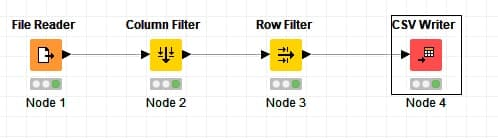
\includegraphics[width=0.9\linewidth]{figuras/capi 1/ejemplo_workflow}
	\caption{Ejemplo de flujo de trabajo en la herramienta KNIME.}
	\label{fig:ejemploworkflow}
\end{figure}
Los metanodos son un tipo de nodo que contiene un subflujo, que pueden contener varios nodos y metanodos \citep{berthold2009knime}, comportándose como un flujo regular. Generalmente se emplea para organizar grandes flujos en varios subflujos que agrupen pequeñas metas, ganando así en claridad. Los componentes en KNIME pueden conformarse por flujos y metanodos, incluso por otros componentes. Estos, a diferencia de los metanodos, poseen la capacidad de configurar parámetros. \\
La herramienta KNIME puede ser extendida a través de plugins, la mayoría son nuevos nodos, aunque las extensiones pueden ser a cualquier parte de la arquitectura. La extensibilidad de la herramienta es de forma sencilla, ya que está basada en la Plataforma de Cliente Enriquecido de Eclipse (\textit{Eclipse RCP}, por sus siglas en inglés) \citep{berthold2009knime}. Gracias a esto, la adición de nuevos plugins a KNIME se torna menos compleja para el desarrollador. \\
KNIME se diseñó en base a tres principios: modularidad, extensibilidad y ambiente de trabajo interactivo. A continuación, se describen estos principios \citep{Lisandra2012}:

\begin{itemize}
	\item Modularidad: Plantea que no deben existir dependencias entre las unidades contenedoras de datos o de procesamiento. Además, se pueden implementar algoritmos de manera independiente. De igual forma, al no tener tipos de datos predefinidos, se pueden definir nuevos tipos de datos, con sus características y especificaciones propias. Estos pueden declararse compatibles con otros existentes.
	\item	Extensibilidad de forma sencilla: Permite adicionar nuevas unidades de procesamiento, visualización y tratamiento de datos, teniendo en cuenta que esto debe ser una tarea fácil de realizar.
	\item	Ambiente de trabajo visual e interactivo: Los flujos de trabajo deben ser fáciles e interactivos para el usuario. Por tal motivo, se harán arrastrando los elementos al área de trabajo.
\end{itemize}

El AutoML en KNIME puede ayudar a simplificar y agilizar el flujo de trabajo de aprendizaje automático, facilitando a los usuarios el desarrollo de modelos predictivos sin necesidad de una intervención manual extensa. Dado que se realiza la modificación a un componente en esta herramienta, se continúa el desarrollo en la misma.

\section{\textit{AutoML} en KNIME}
AutoML en KNIME se refiere a la capacidad de la plataforma para automatizar el proceso de modelado de aprendizaje automático. Esto significa que los usuarios pueden cargar datos y permitir que la plataforma seleccione y optimice automáticamente el modelo que mejor se ajuste a los datos. Con ese objetivo se han desarrollado extensiones y componentes, que permiten a los usuarios de KNIME automatizar tareas de aprendizaje automático, lo que ahorra tiempo y esfuerzo, especialmente para aquellos que pueden no ser expertos en Machine Learning. Sin embargo, al igual que con cualquier herramienta de AutoML, también pueden presentar desafíos, como la selección de algoritmos y la interpretación de modelos. Por lo tanto, es importante comprender las capacidades y limitaciones de las extensiones de AutoML en KNIME y cómo se integran en su flujo de trabajo de análisis de datos antes de su implementación. En las siguientes secciones se analizan de forma breve estas implementaciones.

\subsection{Extensión H2O.ai}
H2O es una plataforma de aprendizaje automático distribuida de código abierto diseñada para escalar a conjuntos de datos muy grandes, con API en R, Python, Java y Scala. H2O AutoML \citep{ledell2020h2o} es un algoritmo automatizado de aprendizaje automático incluido en el marco H2O que es fácil de usar y produce modelos de alta calidad que son adecuados para su implementación en un entorno empresarial. H2O AutoML admite el entrenamiento supervisado de modelos de regresión, clasificación binaria y clasificación multiclase en conjuntos de datos tabulares.\\
H2O.ai, la empresa detrás de H2O AutoML, ha desarrollado una integración con KNIME. Esta permite a los usuarios de la plataforma aprovechar las capacidades de H2O para construir modelos de aprendizaje automático en el entorno de KNIME, lo que facilita la creación de flujos de trabajo de análisis de datos completos, que incluyen tareas de preparación de datos y modelado predictivo. Dentro de la extensión H2O de KNIME, se halla el nodo H2O AutoML, que automatiza el proceso de aprendizaje automático. Este nodo lleva a cabo tareas como el entrenamiento y ajuste automático de diversos modelos, tales como la Máquina de Aumento de Gradiente, el Modelo Lineal Generalizado, las Redes Neuronales Profundas y el Bosque Aleatorio, todo ello dentro de un intervalo de tiempo predeterminado por el usuario. \\
H2O AutoML selecciona el modelo principal y, como parte del proceso de aprendizaje, optimiza automáticamente los hiperparámetros mediante una búsqueda de cuadrícula aleatoria. Además, implementa una validación cruzada con un valor predeterminado de 5 particiones como estrategia de validación. Cabe destacar que este nodo no contiene opciones de pre-procesado de los datos ni permite la visualización ni la modificación de su contenido, únicamente se puede acceder a la interfaz de configuración. Por otra parte, es necesaria la intervención humana para la implementación de los flujos.

\subsection{Componente AutoML KNIME}
Este componente de KNIME, incorporado en el 2021, tiene la capacidad de entrenar automáticamente modelos de aprendizaje automático supervisados para clasificación binaria y multiclase. Automatiza el ciclo de aprendizaje automático, abarcando desde la preparación de datos, la optimización de parámetros con validación cruzada, la puntuación, la evaluación y hasta la selección de modelos. Además, este componente captura de manera integral todo el proceso y genera un flujo de trabajo de implementación mediante la extensión integrada de KNIME. Su funcionamiento se puede resumir de la siguiente manera:

\begin{itemize}
	\item Preparación de datos: Antes de entrenar los modelos, se inicia la fase de preparación de datos. Durante esta etapa, se realiza una limpieza de los datos que implica reemplazar los valores faltantes en las columnas categóricas por la moda y en las columnas numéricas por la media. Existe la opción de aplicar codificación One-Hot a los datos categóricos y de eliminar columnas con un alto número de valores únicos, según un parámetro definido por el usuario. Además, todas las características numéricas se convierten en \textit{double} y se normalizan utilizando la normalización Z-Score. La partición de datos en conjuntos de entrenamiento y prueba se lleva a cabo automáticamente mediante muestreo estratificado en la clase objetivo.
	\item Entrenamiento de modelos: La etapa de entrenamiento de modelos implica la capacitación de diversos tipos de modelos, como Naive Bayes, Regresión Logística, Redes Neuronales, Árboles de Decisión, Bosques Aleatorios y otros. Cada modelo tiene parámetros ajustables que pueden ser optimizados utilizando validación cruzada y una métrica de evaluación personalizada en los datos de entrenamiento. 
	\item Selección del mejor modelo: Una vez que se ha completado el entrenamiento de los modelos, se procede a la selección del mejor. Todos los modelos entrenados se aplican al conjunto de pruebas y se obtienen predicciones. Estas predicciones se comparan con los valores reales, lo que permite calcular diversas métricas de rendimiento. El mejor modelo se selecciona basándose en una métrica de rendimiento especificada por el usuario.
\end{itemize}

Dentro de su configuración, se incluye la selección de los modelos a utilizar, permite seleccionar la partición de entrenamiento y la estrategia de validación, que tiene un valor predeterminado de 5. Sin embargo, debido a su formato caja negra, no se puede visualizar ni modificar los flujos correspondientes a las tareas de AutoML.

\subsection{Componente KNIME de AutoML Clasificación (pre-procesado)}
En \citep{Carrazana2022} se desarrolla un componente KNIME de AutoML para el pre-procesado en tareas de clasificación. Este, a partir de un conjunto de datos y una columna objetivo, ejecuta diferentes flujos de pre-procesado, en aras de cumplir con los requisitos de los diferentes algoritmos de clasificación, siendo capaz de entrenarlos y probarlos, para posteriormente puntuar y graficar los resultados. Este componente está enfocado en el pre-procesado de datos, donde se desarrollaron subcomponentes orientados a la realización de las tareas de pre-procesamiento de datos numéricos, \textit{string}, valores faltantes y el ajuste de tipos de columna. Los algoritmos de clasificación implementados son ID3, C4.5, CART, Redes Neuronales por Retropropagación (RProp), Redes Neuronales Probabilísticas (PNN) y Máquina de Soporte Vectorial (SVM). Cada uno de estos requiere un tipo de pre-procesado diferente, acorde a los tipos de datos con los que trabaja. Este componente consta de tres etapas clave:

\begin{itemize}
	\item Pre-procesado de los datos: Durante esta etapa se ejecutan varios flujos para limpieza de datos, en función de los requerimientos de cada algoritmo implementado. Entre estos flujos se encuentran el ajuste de tipo de columna, para llevar a cabo modificaciones que adecúen los datos al tipo de información que deberían representar; el manejo de columnas de tipo \textit{string}, para eliminar las inconsistencias que se pueden presentar, como caracteres extraños y el uso indistinto de mayúsculas y minúsculas en un mismo valor, así como la eliminación de valores únicos por columna; el manejo de valores faltantes, donde los atributos numéricos y categóricos se sustituyen por la media y moda respectivamente; el tratamiento de valores numéricos, para la conversión de valores nominales en numéricos, y proceder a su normalización, empleando el método Min-Max; y la discretización de variables numéricas, utilizando el método Decimal Scaling.
	\item Entrenamiento de modelos y evaluación: Implica la ejecución de los algoritmos previamente mencionados. En cada cual se ejecuta su evaluación para ser comparados posteriormente, en base a las métricas exactitud y AUC.
	\item Graficado de resultados y selección del modelo: Los resultados obtenidos en la fase anterior se grafican y  el usuario tiene la posibilidad de elegir el que satisfaga sus necesidades. En esta visualización se muestra un grafico de barras con las métricas mencionadas y una curva ROC , para evaluar el rendimiento de los modelos de clasificación. 
\end{itemize}

En su configuración se encuentran la selección de la columna objetivo, los caracteres especiales a eliminar durante el pre-procesado de \textit{string}, el umbral de valores únicos por columna y de valores perdidos permitidos, el porcentaje de partición mediante un muestreo estratificado y la selección de los algoritmos de clasificación que se emplearán. Cabe destacar que este componente permite la visualización y modificación de los flujos implementados. No obstante, a pesar de estar enfocado en el pre-procesado, presenta algunas deficiencias en esta tarea:
\begin{itemize}
	\item Discretización: Este proceso se encuentra estático, es decir, solamente se ejecuta un método de discretización con el nodo AutoBinner, el cual presenta otros métodos que pueden tener un mejor funcionamiento en función de los datos y modelos; incluso, existe otro nodo con el método CAIM para la discretización. Además, esta tarea solo se encuentra implementada en el modelo ID3, cuando C4.5, al ser un árbol de decisión, también trabaja y, a su vez, tolera mejor los datos discretizados.
	\item Normalización: Al igual que la discretización, esta se encuentra de forma estática, cuando en el nodo Normalizer empleado, presenta tres métodos para normalizar. Por otra parte, en este componente solamente está presente la normalización para el modelo Redes Neuronales por Retropropagación; sin embargo, los modelos PNN y SVM, aunque no lo tienen como requisito en la herramienta KNIME, tienen mejor desempeño con los datos normalizados.
	\item Imputación de valores faltantes: El método empleado es la sustitución por la media, en caso de los atributos numéricos, y la sustitución del valor más frecuente, en caso de los valores nominales. Este enfoque, sin estar erróneo, puede sustituirse por la aplicación de métodos de imputación más avanzados, como lo son los que emplean algoritmos de Aprendizaje Automático.
	\item Tratamiento de valores únicos por columna: La interpretación a esta tarea es que, dado un número de valores únicos que existan en una columna de datos nominales, si al contarlos superan este umbral, se eliminen estos valores. No obstante, en este componente se implementa de forma errónea esta tarea, dado que en realidad se cuenta la cantidad de valores distintos que puede tomar un atributo y, si esta cantidad supera a la indicada por el usuario, se elimina la columna. Tras el análisis efectuado en la sección \ref{alta-cardinalidad}, se puede concluir que ambos enfoques afectan el desempeño del modelo.
\end{itemize}
De igual forma, la optimización de hiperparámetros no fue implementada en esta solución, siendo una de las tareas más importantes en AutoML para mejorar el rendimiento de los algoritmos empleados.

\subsection{Análisis comparativo de implementaciones para AutoML en KNIME}
Tras analizar de forma independiente cada uno de estas implementaciones, en la tabla \ref{tab:comparacion-knime} se resumen las mismas, evaluando aspectos fundamentales para su modificación.  La disponibilidad de documentación desempeña un papel crucial, ya que la existencia de recursos claros y accesibles puede determinar la capacidad de los usuarios para comprender y aprovechar al máximo la herramienta. Además, la posibilidad de modificación y adaptación a necesidades específicas es un factor clave, permitiendo a los usuarios personalizar la herramienta según sus requerimientos. El nivel de automatización impacta directamente en la eficiencia del proceso de modelado, lo que es esencial para ahorrar tiempo y recursos. Sin embargo, es importante destacar que todas estas implementaciones presentan desventajas y limitaciones propias, que deben ser consideradas cuidadosamente al tomar una decisión informada sobre la elección de una solución.

% Please add the following required packages to your document preamble:
% \usepackage{booktabs}
% \usepackage{graphicx}
\begin{table}[H]
	\centering
	\caption{Comparativa de las implementaciones para AutoML en KNIME}
	\label{tab:comparacion-knime}
	\begin{spacing}{1.2}
	\resizebox{\textwidth}{!}{%
		\begin{tabular}{@{}lllll@{}}
			\toprule
			Herramienta                                                                                 & \begin{tabular}[c]{@{}l@{}}Disponibilidad de\\ documentación\end{tabular} & \begin{tabular}[c]{@{}l@{}}Nivel de \\ automatización\end{tabular} & \begin{tabular}[c]{@{}l@{}}Posibilidad de\\ modificación\end{tabular} & Desventajas                                                                                                                                                                                                                                 \\ \midrule      \addlinespace[10pt]
			Extensión H2O                                                                               & Limitada                                                                  & Baja                                                               & Media                                                                 & \begin{tabular}[c]{@{}l@{}}- Es necesaria la intervención humana\\ para la implementación de flujos.\\ - No contiene posibilidad de pre-procesado.\end{tabular}                                                                             \\ \addlinespace[10pt]
			Componente AutoML                                                                           & Limitada                                                                  & Alta                                                               & Baja                                                                  & \begin{tabular}[c]{@{}l@{}}- Las actividades de AutoML están \\ predeterminadas.\\ - No se toma en cuenta el algoritmo ni \\ las características de los datos para el \\ pre-procesado.\\ - Funciona en formato de caja negra.\end{tabular} \\ \addlinespace[10pt]
			\begin{tabular}[c]{@{}l@{}}Componente AutoML \\  Clasificación\\ (pre-procesado)\end{tabular} & Asequible                                                                 & Alta                                                               & Alta                                                                  & \begin{tabular}[c]{@{}l@{}}- No esta implementada la optimización \\ de hiperparámetros.\\ - Algunas actividades del pre-procesado\\ están estáticas.\end{tabular}                                                                          \\   \addlinespace[10pt]   \bottomrule
		\end{tabular}%
    	}
		\end{spacing}
\end{table}

Resulta evidente que lo mas factible es continuar el desarrollo del componente AutoML Clasificación (pre-procesado), para lo cual se propone la automatización total del pre-procesado de los datos y la implementación de la optimización de hiperparámetros como parte esencial para mejorar el rendimiento de los modelos de aprendizaje automático, ahorrar tiempo y recursos, aumentar la robustez, adaptarse a cambios en los datos y avanzar en la investigación y el desarrollo de algoritmos. A lo largo de los próximos epígrafes, se abordarán en profundidad las tareas previamente mencionadas. \\
Durante el transcurso de esta investigación, el componente AutoML de KNIME fue actualizado, a la fecha del 20 de octubre de 2023 \citep{KNIME2023-11}. Estas actualizaciones incluyen algunas mejoras, donde la más relevante es el acceso a los flujos implementados y su modificación. No obstante, tras analizar a más detalle el funcionamiento del componente, se encuentra que se mantiene la predeterminación de las tareas de AutoML. Por ejemplo, la estrategia de optimización de hiperparámetros está establecida a Búsqueda Aleatoria, y para cambiar esta configuración, la única posibilidad es que el usuario se adentre en los flujos implementados; siendo el mismo problema en la etapa del pre-procesado con las actividades de discretización, normalización y manejo de valores faltantes. Por otra parte, el pre-procesado específico de cada algoritmo no se toma en cuenta, lo cual es fundamental en la etapa de preparación de los datos. Asimismo, no se incluyen hiperparámetros que si se toman en cuenta en el desarrollo de esta investigación.


\begin{comment}
	\section{Componente KNIME de AutoML para el pre-procesado en tareas de clasificación}\label{epig:componente-ernesto}
	Con tal objetivo, en \citep{Carrazana2022} se desarrolla un componente KNIME de AutoML para el pre-procesado en tareas de clasificación. Este, a partir de un conjunto de datos y una columna objetivo, ejecuta diferentes flujos de pre-procesado, en aras de cumplir con los requisitos de los diferentes algoritmos de clasificación, siendo capaz de entrenarlos y probarlos, para posteriormente puntuar y graficar los resultados \citep{Carrazana2022}. En el anexo \ref{anex:flujo-automl-componente} se muestra el flujo KNIME del Componente AutoML Clasificación (pre-procesado). \\
	Este componente está enfocado en el pre-procesado de datos, donde se desarrollaron subcomponentes enfocados en la realización de las tareas de pre-procesamiento de datos numéricos, \textit{string}, valores faltantes y el ajuste de tipos de columna. Como se observa en el anexo \ref{anex:flujo-automl-componente}, se aplican los algoritmos de clasificación ID3, C4.5, CART, Redes Neuronales por Retropropagación (RProp), Redes Neuronales Probabilísticas (PNN) y Máquina de Soporte Vectorial (SVM). Cada uno de estos requiere un tipo de pre-procesado diferente, acorde a los tipos de datos con los que trabaja. \\
	
	En los siguientes epígrafes se profundiza en estas dos tareas de vital importancia para el AutoML: el pre-procesado y la optimización de hiperparámetros. 
\end{comment}


\section{Pre-procesado} \label{epig:preprocesado}
Una tarea importante en el proceso de AutoML es el pre-procesamiento de datos, siendo el conjunto de técnicas utilizadas para preparar los datos de entrada antes de alimentarlos a un modelo de aprendizaje automático. Esta etapa es la equivalente a la fase de selección, limpieza y transformación del proceso de KDD, descrita brevemente en la sección \ref{kdd}. \\
El pre-procesamiento de datos ayuda a mejorar la calidad de los datos de entrada y puede mejorar el rendimiento del modelo. La automatización del pre-procesamiento de datos a través de herramientas de AutoML, puede mejorar la eficiencia del proceso y ayudar al personal especializado, o sin mucha experiencia en el campo, a trabajar de manera más efectiva. Entre las técnicas de pre-procesado de datos se encuentran la discretización, la normalización, el tratamiento de valores faltantes y de atributos de tipo \textit{string}.

\subsubsection*{Discretización} \label{sub-epigrafe-disc}
Este procedimiento transforma datos cuantitativos en datos cualitativos, es decir, atributos numéricos en atributos discretos o nominales con un número finito de intervalos, obteniendo una partición no superpuesta de un dominio continuo. Luego se establece una asociación entre cada intervalo con un valor numérico discreto. Una vez realizada la discretización, los datos pueden ser tratados como datos nominales durante cualquier proceso de minería de datos \citep{garcia2015data}, \citep{garcia2012survey}. \\
Es necesario realizar la discretización de variables porque, entre varios factores, muchos de los algoritmos de Aprendizaje Automático requieren el uso de valores nominales solamente, como es el caso de ID3, Redes Bayesianas y Apriori. Otras ventajas derivadas de la discretización son la reducción y simplificación de datos, agilizando el aprendizaje y arrojando resultados más precisos, compactos y breves; y se reduce el posible ruido presente en los datos \citep{garcia2012survey}. No obstante, cualquier proceso de discretización conlleva generalmente una pérdida de información, siendo la minimización de esta pérdida el objetivo principal de un discretizador. \\
La elección del número de bins o intervalos para la discretización de datos es un proceso importante en el análisis de datos cuantitativos. El número de bins determina cómo se agrupan los valores continuos en categorías o intervalos discretos y puede influir en la interpretación de los resultados. Normalmente, este número es a elección del usuario, a pesar de que no existe una regla única para determinar el número de bins. En la literatura se han encontrado otros métodos, como:
\begin{itemize}

	\item Regla de Sturges \citep{coria2013mineria}: Propuesta por Herbert Sturges en 1926 \citep{sturges1926choice}, es una regla práctica para la selección del número de clases que se deben considerar al elaborar un histograma. Este número (\textit{k}) viene dado por la fórmula \ref{sturges}, donde \textit{n} es el tamaño de la muestra.
	\begin{equation} \label{sturges}
		k = 1 + \log_{2} n
	\end{equation}

	\item Validación cruzada \citep{torgo1997search}: La idea básica es probar diferentes configuraciones de parámetros y elegir la que proporcione la mejor precisión estimada. Esta mejor configuración encontrada se utilizará luego en el algoritmo de aprendizaje en la evaluación real, utilizando un conjunto de pruebas independiente. En cuanto al componente de búsqueda, se utiliza el escalador de colinas (hill-climbing) junto con un parámetro de anticipación configurable para minimizar el conocido problema de los mínimos locales. Para la estrategia de validación se emplea la validación cruzada.

	\item Tamaño de la muestra \citep{dougherty1995supervised}: Se calcula k teniendo en cuenta el número de valores distintos observados en el conjunto de entrenamiento, utilizando
	\begin{equation}
		k = max(1, 2 * \log l )
	\end{equation}
	 donde \textit{l} es el número de valores distintos observados para cada atributo.

\end{itemize}

La identificación del mejor discretizador para cada situación es una tarea muy difícil de llevar a cabo. A pesar de la riqueza de la literatura, y aparte de la ausencia de una categorización completa de los discretizadores usando una notación unificada, hay pocos intentos de compararlos empíricamente. Esto se debe a que la evaluación de resultados es un tema complejo y depende de la necesidad del usuario en una aplicación en particular; además, la evaluación se puede hacer de muchas maneras. Existen tres dimensiones importantes según \citep{liu2002discretization}: 
\begin{enumerate}
	\item El número total de intervalos: intuitivamente, cuantos menos puntos de corte, mejor será el resultado de la discretización.
	\item El número de inconsistencias causadas por la discretización: no debe ser mucho mayor que el número de inconsistencias de los datos originales antes de la discretización.
	\item Precisión predictiva: cómo la discretización ayuda a mejorar la precisión.
\end{enumerate}
En resumen, se necesitan al menos tres dimensiones: simplicidad, consistencia y precisión. Idealmente, el mejor resultado de discretización puede obtener la puntuación más alta en los tres departamentos. En realidad, puede no ser alcanzable o necesario. Existen diversos algoritmos y enfoques utilizados para realizar esta conversión:

\begin{itemize}
	
	\item Agrupamiento (binning): es el método más simple para discretizar un atributo de valor continuo mediante la creación de un número específico de grupos (bins). Los bins se pueden crear con el mismo ancho (\textit{equal-width}) o la misma frecuencia (\textit{equal-frequency}). Cada bin está asociado con un valor discreto distinto. En \textit{equal-width}, el rango continuo de una característica se divide uniformemente en intervalos que tienen un ancho igual, y cada intervalo representa un bin. En \textit{equal-frequency}, se coloca un número igual de valores continuos en cada bin \citep{liu2002discretization}, \citep{yang2009discretization}. 
	
	\item Basado en cuantiles (\textit{quantiles-based}): Un método simple y similar a los anteriores, donde se producen bins correspondientes a una lista de probabilidades dada. El elemento más pequeño corresponde a una probabilidad de 0 y el más grande a una probabilidad de 1. 
	
	\item CAIM (Clustering and Mutual Information): El objetivo es encontrar el número mínimo de intervalos discretos mientras se minimiza la pérdida de interdependencia de atributo de clase. El algoritmo utiliza información de interdependencia de atributo de clase como criterio para la discretización óptima \citep{kurgan2004caim}. 
	
\end{itemize}

Existen otros métodos, que según el estudio realizado en \citep{garcia2012survey} son los más empleados, aparte de los mencionados anteriormente, como MDLP \citep{FI1993}, ID3 \citep{quinlan1993c}, ChiMerge \citep{K1992}, 1R \citep{holte1993very}, D2 \citep{catlett1991changing}, y Chi2 \citep{liu1997feature}. Sin embargo, en este contexto de investigación, es importante destacar que estos no serán empleados para la discretización de los atributos. La decisión se basa en la disponibilidad de implementaciones en KNIME de los métodos de agrupamiento, el basado en cuantiles (quantiles-based) y el algoritmo CAIM. Esta selección se realiza en consonancia con la revisión de la literatura y la investigación existente en el campo.

\subsubsection*{Normalización}
Las variables del conjunto de datos pueden variar en términos de magnitud, rango y unidad. Esto puede afectar negativamente el rendimiento de algoritmos, como SVM y redes neuronales, que emplean, en su mayoría, datos numéricos. En aras de resolver este problema, se realiza la normalización. Esta consiste  en ajustar los valores de una variable para que estén dentro de un rango específico o sigan una distribución particular. Se ejecuta principalmente para garantizar que las diferencias en la escala de las variables no afecten negativamente el rendimiento de los algoritmos de aprendizaje automático; y para facilitar la interpretación de los datos.\\
Existen varias técnicas de normalización comunes, donde algunas de las más utilizadas son la normalización Min-Max, Z-Score y Escala Decimal \citep{garcia2012survey}. En la literatura se pueden encontrar otras técnicas, descritas a continuación:
\begin{itemize}
	\item Normalización Min-Max: Transforma los valores de una variable para que estén en un rango específico, generalmente entre 0 y 1. Desventaja: Es sensible a valores atípicos.
	\item Normalización Z-score (estandarización): Transforma los valores para que tengan una media de 0 y una desviación estándar de 1. Desventaja: No escala los valores a un rango específico.
	\item Normalización de Escala Decimal: Transforma los valores desplazando el punto decimal, usando una división de potencia de diez, de modo que el valor absoluto máximo sea siempre inferior a 1 después de la transformación. Desventaja: Puede llevar a una pérdida significativa de precisión en los valores pequeños. 
	\item Normalización sólida \citep{polatgil2022investigation}: Este método es más útil especialmente cuando hay un valor atípico en los datos porque utiliza el valor mediano en lugar de la media y el rango de cuartiles en lugar del rango de valores. Sin embargo, la desventaja es que esta reducción de influencia de valores atípicos puede llevar a una pérdida de sensibilidad a la variabilidad de los datos.
	\item Escalador de Máximo Absoluto (Max Abs): En este método cada característica de los datos se obtiene dividiendo su valor máximo absoluto \citep{polatgil2022investigation}. Desventaja: No escala los valores a un rango específico, lo que puede dificultar la interpretación.
	\item Normalización AMZD: Propuesta en \citep{patro2015normalization} y similar a Min-Max, transforma los valores de datos de manera que tengan una representación en un rango de 0 y 1, con la diferencia de que funciona a nivel individual, lo que significa que se aplica a cada elemento de datos por separado; es independiente del tamaño del conjunto de datos; y
	es independiente del número de dígitos en cada elemento de datos. Sin embargo,  presenta como desventaja que solo puede ser aplicada a datos enteros.
\end{itemize}

 En el contexto de AutoML (Aprendizaje Automático Automatizado), donde se busca una automatización eficiente del proceso de construcción de modelos, es crucial identificar un normalizador que sea coherente con los algoritmos utilizados. Algunos algoritmos pueden ser más sensibles a la escala y la distribución de las variables que otros. Por lo tanto, en esta investigación se realizan experimentos para evaluar el rendimiento de los modelos con diferentes técnicas de normalización y se selecciona la que maximice la calidad de las predicciones. En el capítulo \ref{chap:2} se profundiza en esta tarea.
 
\subsubsection*{Tratamiento de valores faltantes} \label{secc:mv}
Los valores faltantes o perdidos son datos que no aparecen en la celda de la columna que les corresponde. Esto puede ocurrir por diversas razones, como errores en la recolección de datos, omisiones intencionales, fallos en la medición o simplemente porque no se disponía de información en el momento de la recopilación. Esto trae consigo varias dificultades: disminución de la eficacia, complicaciones en la gestión y análisis de datos; así como a resultados sesgados. Sin embargo, los datos incompletos son objeto de investigación debido a su influencia en la precisión de la clasificación. Normalmente, los valores perdidos pueden ser manejados de varios métodos \citep{garcia2015data}, \citep{ventevogel2020construction}:
\begin{itemize}
	\item Descartar los valores: Consiste en eliminar por completo los registros que contienen valores faltantes. Descartar completamente un atributo es un enfoque que se puede utilizar cuando se observan muchos valores perdidos para el mismo. Una regla general es que si faltan más del 60-70\% de los valores, es mejor eliminar el atributo \citep{ventevogel2020construction}. Sin embargo, este método puede resultar en la pérdida de información valiosa y reducir el tamaño de la muestra.
	\item Imputación mediante muestreo: Este enfoque es más adecuado para funciones no categóricas. Al aplicarlo, se utilizan procedimientos de máxima verosimilitud para estimar los parámetros de la porción completa de los datos. Utilizando estos parámetros, los valores perdidos se completan mediante muestreo de esta distribución estimada.
	\item Imputación múltiple: Implica reemplazar los valores faltantes por un valor constante, como la media, la mediana o la moda de la variable en cuestión. Este enfoque es útil cuando los valores faltantes son aleatorios y no se espera que sigan un patrón específico. Para datos faltantes más complejos, es posible utilizar modelos predictivos para estimar los valores perdidos. Esto puede incluir regresiones, árboles de decisión o métodos de Machine Learning más avanzados.
\end{itemize}
En el contexto de este análisis, nos enfocamos en este último método. Existe una amplia familia de métodos de imputación, desde técnicas de imputación simples como sustitución de medias, KNN, etc.; a aquellos que analizan las relaciones entre atributos tales como: basados en SVM, basados en clustering, regresiones logísticas, procedimientos de máxima verosimilitud e imputación múltiple. En esta investigación se emplean los métodos KNN y K-Means para la imputación de estos valores, dado que en KNIME se tiene la posibilidad de implementarlos y en la literatura se ha demostrado que son robustos para esta tarea \citep{tsai2022empirical}, \citep{batista2003analysis}, \citep{patil2010missing}, \citep{li2004towards}.\\
K-Vecinos Más Cercanos (K-Nearest Neighborst o KNN) es un algoritmo de aprendizaje supervisado, que se utiliza comúnmente para la imputación de valores faltantes en conjuntos de datos. La idea básica es encontrar las \textit{k} observaciones más cercanas a la observación con el valor faltante, y utilizar los valores de esas observaciones para estimar el valor faltante. \\
Por otra parte, K-Medias (K-Means) es un algoritmo de aprendizaje no supervisado que se utiliza para la agrupación de datos. Se puede usar como parte de un enfoque más amplio para la imputación, por ejemplo, para agrupar observaciones similares y luego imputar valores faltantes dentro de cada grupo utilizando técnicas específicas, como la imputación de la media o la mediana del grupo.

\subsubsection*{Tratamiento de atributos de alta cardinalidad}\label{alta-cardinalidad}
Los atributos categóricos, en contraste con los atributos numéricos, representan categorías o etiquetas. Se dividen en dos tipos principales: nominales, que representan categorías sin orden específico (como colores o países), y ordinales, que muestran un orden jerárquico (como niveles educativos). En muchos conjuntos de datos, es común encontrarse con atributos categóricos que presentan una alta cardinalidad. La cardinalidad de un atributo categórico esta definida por el número de valores distintos que un atributo puede tomar \citep{moeyersoms2015including}. Las variables categóricas de alta cardinalidad son variables para las cuales el número de niveles diferentes es grande en relación con el tamaño de la muestra de un conjunto de datos. \\
Estos atributos presentan desafíos significativos en el análisis de datos y requieren un manejo cuidadoso. Uno de los problemas clave que se enfrentan es la complejidad computacional, ya que una gran cantidad de categorías puede aumentar el tiempo de procesamiento y el consumo de memoria. Además, pueden llevar a problemas de sobreajuste en modelos de aprendizaje automático y dificultar la interpretación de resultados. Por ejemplo, en un país existen muchos importadores y exportadores diferentes. Al entrenar un modelo de aprendizaje automático, este tipo de datos no son útiles, ya que dificulta la generalización del modelo, pero con un método de codificación adecuado, se ha demostrado que estas características mejoran el rendimiento del modelo de clasificación \citep{hooi2022feature}, \citep{cerda2020encoding}. Para abordar estos problemas, existen varias estrategias, como el agrupamiento semántico, que consiste en identificar grupos significativos desde el punto de vista semántico \citep{cerda2018similarity}; y distintos métodos de codificación, como One-Hot, Target, Peso de Evidencia (WOE) y Radio Supervisado. \\
One-Hot Encoding transforma una característica categórica de \textit{q} categorías únicas en representaciones numéricas, construyendo \textit{q} atributos binarios, uno para cada categoría; \citep{avanzi2023machine}. En el ejemplo de la figura \ref{fig:one-hot-ejemplo}, los códigos ZIP de clientes individuales (C1, C2, etc.) se transforman utilizando este método, donde se crea una variable  para cada código ZIP. \\
En otras palabras, cada dimensión representa la ausencia o presencia de una categoría dada. En \citep{hooi2022feature} se realizan pruebas para comparar el desempeño de varias técnicas de codificación con respecto a algoritmos de Aprendizaje Automático, como SVM, árboles de decisión y redes neuronales, lo cual, con respecto al codificador One-Hot, se obtuvieron muy buenos resultados. \\
\begin{figure}[H]
	\centering
	\includegraphics[width=0.8\linewidth]{"figuras/capi 1/one-hot-ejemplo"}
	\caption{Ejemplo de One-Hot Encoding (también conocido como Dummy Encoding) para el atributo ZIP Code}
	\label{fig:one-hot-ejemplo}
\end{figure}
Este método, aunque eficaz para atributos de baja cardinalidad, presenta la desventaja de generar una alta dimensionalidad, lo que puede ocasionar desafíos computacionales y estadísticos. Para evitarlo, es necesario aplicar reducción de dimensionalidad en la matriz de características resultante. Un enfoque natural es utilizar el Análisis de Componentes Principales (PCA) \citep{mahmood2022accurate}, \citep{kasemtaweechok2021large} , donde la idea básica es encontrar un conjunto de transformaciones lineales de las variables originales que puedan describir la mayor parte de la varianza utilizando un número relativamente menor de variables \citep{garcia2015data}. Este enfoque permite la combinación de la esencia de los atributos originales para formar un nuevo subconjunto más pequeño de atributos. \\
La reducción de la cardinalidad comprende las transformaciones aplicadas para obtener una representación reducida de los datos originales. Un ejemplo de reducción de cardinalidad es la introducción de un valor \textit{otros}, que se asigna a los valores que representan menos de un cierto umbral en el atributo \citep{casas2019data}. Esto es especialmente útil cuando muchos valores ocurren muy pocas veces \citep{ventevogel2020construction}.

\section{Optimización de hiperparámetros} \label{epig:hpo}
La optimización de hiperparámetros es un componente esencial en el campo del aprendizaje automático. En el proceso de entrenar modelos, los hiperparámetros desempeñan un papel crítico al influir en el rendimiento y la capacidad de generalización de un algoritmo. La tarea de optimizar estos hiperparámetros implica encontrar la combinación óptima que maximice la eficiencia, precisión y rendimiento de un modelo en un conjunto de datos de prueba o validación  \citep{hastie2009elements}. La optimización de hiperparámetros automatizada (HPO) tiene varios casos de uso importantes  \citep{hutter2019automated}; puede
\begin{itemize}
	\item reducir el esfuerzo humano necesario para aplicar el aprendizaje automático. Particularmente importante en el contexto de AutoML,
	\item mejorar el rendimiento de los algoritmos de aprendizaje automático (adaptándolos al problema en cuestión), y
	\item mejorar la reproducibilidad y equidad de los estudios científicos.
\end{itemize}
Para ahorrar tiempo y mejorar la precisión de los modelos de aprendizaje automático, se combina la selección de algoritmos y la optimización de hiperparámetros en un solo proceso, denominado Selección de Algoritmos y Optimización de Hiperparámetros Combinados (\textit{CASH}, por sus siglas en inglés) \citep{tuggener2019automated}. \\
CASH, en conjunción con la automatización del pre-procesado de los datos, integran el problema general del AutoML, reflejado en la figura \ref{fig:desglose-de-los-subproblemas-de-automl}. 
\begin{figure}[H]
	\centering
	\includegraphics[width=0.6\linewidth]{"figuras/capi 1/Desglose de los subproblemas de AutoML"}
	\caption{Desglose de los subproblemas de AutoML \citep{zoller2021benchmark}}
	\label{fig:desglose-de-los-subproblemas-de-automl}
\end{figure} 
Existen varias estrategias de HPO, algunas de las cuales son:
\begin{itemize}
	\item Búsqueda aleatoria: Selecciona valores de forma aleatoria dentro de un rango definido. No garantiza encontrar los mejores valores posibles, y puede requerir numerosas iteraciones para encontrar un conjunto de hiperparámetros que proporcione un rendimiento óptimo \citep{geron2022hands},\citep{zoller2021benchmark}.
	\item Búsqueda voraz: Prueba todas las combinaciones posibles de valores de los hiperparámetros dentro de un rango definido. Presenta una alta demanda computacional, imposible de manejar a medida que escalan los sistemas y las bases de datos \citep{zoller2021benchmark}.
	\item Búsqueda en cuadrícula: Prueba cada combinación de valores de hiperparámetros y selecciona la combinación que haya dado el mejor rendimiento. Puede ser computacionalmente costoso si el espacio de búsqueda y el número de hiperparámetros es grande \citep{he2021automl}.
	\item Optimización Bayesiana: Construye modelos probabilísticos para representar la función objetivo, que se actualiza después de cada iteración. Maneja espacios de búsqueda de alta dimensionalidad, y no requiere tantas iteraciones, como la búsqueda en cuadrícula o la búsqueda aleatoria, para encontrar combinaciones de hiperparámetros de alto rendimiento \citep{hutter2019automated}, \citep{he2021automl}.
	\item Optimización basada en gradiente: Emplea la información del gradiente para optimizar los hiperparámetros de manera iterativa. Genera una gran carga computacional y presenta la limitación de caer en mínimos locales \citep{zoller2021benchmark}.
\end{itemize} 

Una vez identificadas las variables clave del modelo, es crucial evaluar su rendimiento de manera sólida y confiable. En este contexto, las técnicas de validación son una herramienta esencial para evaluar y comparar diferentes combinaciones de hiperparámetros. Para lograr esto, una técnica esencial es la validación cruzada. La validación cruzada implica dividir el conjunto de datos en múltiples subconjuntos, entrenando y evaluando el modelo en diferentes particiones para estimar su capacidad de generalización. Esta estrategia nos permite determinar cómo se comporta el modelo con diferentes combinaciones de datos de entrenamiento y prueba, lo que es especialmente importante cuando se trata de la selección de hiperparámetros y la evaluación de su impacto en el rendimiento \citep{hastie2009elements}. \\
A pesar del incesante estudio vinculado al HPO, este sigue presentando en la actualidad diversos desafíos \citep{hutter2019automated}:
\begin{itemize}
	\item Costo computacional: la optimización de hiperparámetros puede ser muy costosa en términos de tiempo de cómputo y recursos de hardware, especialmente cuando se utiliza un espacio de hiperparámetros grande o se ejecutan muchas iteraciones de entrenamiento. Esto puede limitar la escalabilidad y la eficiencia de la HPO.
	\item Generalización del modelo: la optimización de hiperparámetros puede resultar en un modelo altamente ajustado, que no generaliza bien a nuevos datos. Se torna complejo cuando las bases de datos poseen múltiples tipos de datos.
	\item Complejidad del espacio de hiperparámetros: el espacio de hiperparámetros puede ser muy complejo y estar altamente interconectado, lo que dificulta la exploración y la selección de los hiperparámetros adecuados.
\end{itemize}

Entre las aplicaciones de HPO, se pueden encontrar dos ejemplos destacados en la literatura. En primer lugar, \citep{hernandeztecnicas} aplica HPO en SVM y bosques aleatorios para predecir enfermedades cardiovasculares. En segundo lugar, \citep{waring2020automated} aborda el desarrollo del problema de HPO en redes neuronales en un contexto de análisis de salud.


\section{Clasificación}
En el uso común, la palabra clasificación significa colocar las cosas en categorías, agruparlas de alguna manera útil. El ser humano generalmente hace esto porque las cosas en un grupo, llamado \textit{clase} en aprendizaje automático, comparten características comunes \citep{sammut2011encyclopedia}. \\
En aprendizaje automático, la clasificación se utiliza para identificar a qué clase o categoría pertenece una determinada observación o registro, basándose en un conjunto de características o variables. En esta tarea, se utiliza un algoritmo para construir un modelo predictivo que asigne una etiqueta de clase a cada observación en función de sus características. Este modelo se entrena utilizando un conjunto de datos etiquetados previamente, y luego se aplica a nuevos datos para hacer predicciones \citep{sammut2011encyclopedia}. En las siguientes secciones se describen los algoritmos empleados en el componente AutoML Clasificación (pre-procesado).

\subsubsection{Clasificación con Árboles de Decisión}
La clasificación con árboles de decisión es un método popular en la minería de datos y en el aprendizaje automático supervisado, utilizado para predecir la clase o categoría de un objeto o registro. Los Árboles de Decisión son unos de los modelos más populares, su representación es de fácil entendimiento, incluso por personas no afines al área, pues su construcción en sencilla: las hojas toman los valores objetivos, mientras los atributos y sus posibles valores conforman los nodos y ramas respectivamente \citep{sammut2011encyclopedia}. \\
Basados en árboles de decisión existen otros algoritmos de clasificación como: ID3, C4.5 y CART. Cada uno de ellos fue desarrollado como una versión mejorada del anterior, pero todos tienen una alta eficiencia y tiempos de ejecución reducidos, lo que los hace igualmente populares en la actualidad \citep{javed2022performance}. Por otra parte, el algoritmo Bosque Aleatorio (mejor conocido como Random Forest, por su traducción al inglés), se basa en la idea de combinar múltiples árboles de decisión para mejorar la precisión y la capacidad de generalización del modelo. Se comparan y analizan en \citep{gupta2017analysis}, donde se arrojan sus principales características:
\begin{itemize}
	\item ID3 (Iterative Dichotomiser 3): Basa su funcionamiento en la entropía y la ganancia de información. El árbol se construye iterativamente de arriba hacia abajo, eligiendo en cada caso el atributo con mayor ganancia de información, hasta que la información ganada sea cero o se haya llegado a todas las hojas \citep{javed2022performance}, \citep{gupta2017analysis}. Maneja datos nominales y no tolera valores faltantes.
	\item C4.5 (Classification 4.5): Desarrollado con el objetivo de mejorar los defectos de ID3. Añade la poda, desestimando las ramas sin aportes, que reduce los errores al clasificar como resultado de un gran número de ramas en el modelo \citep{sammut2011encyclopedia}, \citep{javed2022performance}, \citep{gupta2017analysis}. Adicionalmente maneja valores faltantes y numéricos. 
	\item CART (Classification and Regression Trees): Genera un árbol binario siguiendo el mismo enfoque entrópico que ID3, pero empleando el coeficiente de Gini como criterio de selección \citep{javed2022performance}, \citep{gupta2017analysis}. Es capaz de manejar datos faltantes, al igual que datos numéricos y nominales.
	\item Random Forest: Es un algoritmo de aprendizaje automático en el que se construye un conjunto de árboles de decisión para realizar predicciones. Cada árbol se entrena con un subconjunto aleatorio de datos y características, y luego se combina su salida para obtener una predicción más robusta y precisa. Reduce el sobreajuste y mejora la generalización al promediar múltiples modelos \citep{gupta2017analysis}.
\end{itemize}

\subsubsection{Clasificación con Redes Neuronales}
Las redes neuronales o redes neuronales artificiales, son algoritmos de aprendizaje basados en una vaga analogía de cómo funciona el cerebro humano. El aprendizaje se logra ajustando los pesos en las conexiones entre nodos, que son análogas a las sinapsis y las neuronas \citep{sammut2011encyclopedia}. \\
Las primeras redes neuronales conocidas como pre-alimentadas, como la de la figura \ref{fig:red-neuronal-prealimentada}, se caracterizan por tener una arquitectura en la que cada capa de neuronas está conectada completamente con la capa siguiente, pero no con la capa anterior. Esto significa que la información fluye de forma unidireccional, sin retroalimentación \citep{abiodun2018state}. 
\begin{figure}[H]
	\centering
	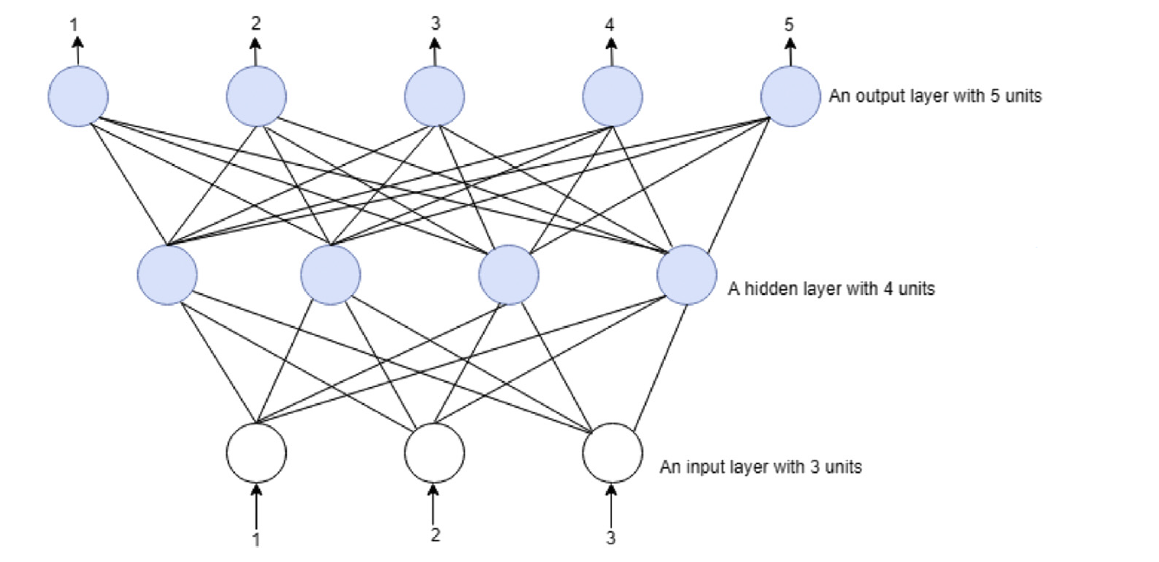
\includegraphics[width=0.7\linewidth]{figuras/capi 1/red-neuronal-prealimentada}
	\caption{Red Neuronal Pre-Alimentada \citep{abiodun2018state}}
	\label{fig:red-neuronal-prealimentada}
\end{figure}
Posteriormente, se desarrollaron las redes neuronales por retro-propagación, como la presente en la figura \ref{fig:red-neuronal-retropropagacion}, que comparan la salida obtenida por la red con la salida deseada, y ajustan los pesos de las conexiones entre las neuronas de la red para reducir el error de predicción. La retro-propagación se utiliza para calcular la contribución de cada peso en el error de la red, y así ajustarlos de manera adecuada \citep{abiodun2018state}.
\begin{figure}[H]
	\centering
	\includegraphics[width=0.6\linewidth]{figuras/capi 1/red-neuronal-retropropagación}
	\caption{Red neuronal por retro-propagación \citep{abiodun2018state}}
	\label{fig:red-neuronal-retropropagacion}
\end{figure}
Gracias a su gran versatilidad se pueden aplicar en una amplia variedad de campos y disciplinas para resolver problemas complejos de aprendizaje automático, como es el procesamiento del lenguaje natural, reconocimiento de voz e imágenes \citep{abiodun2018state}. Debido a la complejidad de sus modelos puede ser difícil su entendimiento, por lo que preferiblemente se utilizan en el contexto del reconocimiento de patrones.

\subsubsection{Clasificación con Support Vector Machine}
Las Máquinas de Soporte Vectorial (Support Vector Machine o SVM, en inglés), son una clase de algoritmos lineales que se pueden emplear para la clasificación \citep{sammut2011encyclopedia}, cuyo objetivo es encontrar el hiperplano que mejor separa dos clases de datos en un espacio de alta dimensionalidad \citep{guenther2016support}. En la figura \ref{fig:ejemplos-de-posibles-hiperplanos-de-svm} se representa como el hiperplano H2 divide con mayor margen las clases que el hiperplano H1.
\begin{figure}[H]
	\centering
	\includegraphics[width=0.4\linewidth]{"figuras/capi 1/Ejemplos de posibles hiperplanos de SVM"}
	\caption{Ejemplos de posibles hiperplanos de SVM \citep{sammut2011encyclopedia}}
	\label{fig:ejemplos-de-posibles-hiperplanos-de-svm}
\end{figure}
Uno de los desafíos de SVM en problemas de clasificación de múltiples clases es cómo manejar la predicción de estas. En este contexto, existen dos enfoques principales:
\begin{itemize}
	\item Uno contra uno (One-vs-One): Durante la fase de predicción, cada clasificador binario vota por la clase que cree que es correcta y la clase con el mayor número de votos se selecciona como la clase final para el punto de datos dado. Este enfoque presenta la ventaja de que cada clasificador binario solo necesita ser entrenado en un subconjunto de los datos, lo que puede ser útil cuando hay grandes conjuntos de datos. Es más resistente a desequilibrios en la distribución de clases que otros enfoques de SVM \citep{guenther2016support}.
	\item Uno contra todos (One-vs-All): Entrena un clasificador binario para cada clase posible, donde el conjunto de datos de una clase se considera positivo y los datos de las otras clases se consideran negativos. Durante la fase de predicción, cada clasificador binario vota por su clase correspondiente y la clase con la mayor puntuación se selecciona como la clase final para el punto de datos dado. Fácil de implementar y puede funcionar bien en conjuntos de datos pequeños, pero puede ser menos preciso en conjuntos de datos grandes y complejos \citep{guenther2016support}.
\end{itemize}
Agregar que existen otros dos enfoques: Clasificación jerárquica (Hierarchical classification) y Clasificación por parejas (Pairwise classification). Cada uno de estos tiene sus propias ventajas y desventajas, y la elección de uno de ellos dependerá del tipo de datos y del problema que se esté tratando de resolver. Es importante mencionar que la clasificación es solo una de las muchas técnicas utilizadas en el Aprendizaje  Automático. 

\section{Métodos para la evaluación en clasificación}
En el campo de la clasificación, existen varios métodos de evaluación que se utilizan para comparar diferentes algoritmos o enfoques en esta tarea. Estos métodos ayudan a medir el rendimiento y la eficacia de los modelos de clasificación, así como a tomar decisiones informadas sobre cuál es el mejor enfoque para una tarea específica. Cuando se trabaja en problemas de clasificación con atributos numéricos, es fundamental contar con una base de datos de prueba adecuada. Una buena base de datos debe ser representativa de los datos del mundo real, y contener una variedad de instancias y etiquetas de clase para evaluar el rendimiento de los algoritmos de clasificación.

\subsection{Bases de datos de prueba}
Las bases de datos de prueba son conjuntos de datos creados para ayudar a los desarrolladores a probar y depurar aplicaciones de bases de datos, sin tener que utilizar datos reales y confidenciales. Estas bases de datos contienen datos ficticios, pero siguen la estructura de una base de datos real, lo que permite a los desarrolladores probar la funcionalidad de la aplicación sin preocuparse por dañar datos importantes o comprometer la privacidad de los usuarios. Kaggle Datasets\footnote{https://www.kaggle.com/datasets} y UCI Machine Learning Repository\footnote{https://archive.ics.uci.edu/datasets} son dos de los repositorios en línea más populares para conjuntos de datos de prueba y de aprendizaje automático. \\
Kaggle Datasets es un sitio web de aprendizaje automático que ofrece una amplia variedad de conjuntos de datos de muestra, desde datos meteorológicos hasta datos de redes sociales. Los usuarios pueden buscar entre miles de conjuntos de datos y también pueden contribuir con los propios. Kaggle también tiene una comunidad de científicos de datos y aprendizaje automático, que pueden proporcionar comentarios y ayudar a los usuarios a mejorar sus modelos de aprendizaje automático. \\
Por otro lado, el UCI Machine Learning Repository es un repositorio de conjuntos de datos de muestra para aprendizaje automático, minería de datos y otras aplicaciones de análisis de datos. El repositorio fue creado por la Universidad de California, Irvine, y contiene una amplia gama de conjuntos de datos, desde reconocimiento de voz hasta predicción de precios de viviendas. Los usuarios pueden descargar los conjuntos de datos de forma gratuita y utilizarlos para probar y desarrollar sus modelos de aprendizaje automático. \\
Ambos repositorios ofrecen una amplia variedad de conjuntos de datos, lo que los hace ideales para desarrolladores, estudiantes y profesionales de la ciencia de datos que buscan mejorar sus habilidades en el modelado de bases de datos y en la creación de modelos de aprendizaje automático precisos y efectivos. Por tal motivo, se emplearán ambos repositorios para la obtención de bases de datos para las pruebas que se realizarán en esta investigación.

% Please add the following required packages to your document preamble:
% \usepackage{booktabs}
% \usepackage{graphicx}
\begin{table}[H]
	\centering
	\caption{Bases de datos empleadas en la experimentación}
	\label{tab:bd-cap1}
	\begin{spacing}{1.2}
	\resizebox{\textwidth}{!}{%
		\begin{tabular}{@{}ccccccc@{}}
			\toprule
			Base de datos   & \#Instancias & \begin{tabular}[c]{@{}c@{}}\#Atributos\\ (cuantitativos, cualitativos)\end{tabular} & Clases                                                                      & \%Clases                                                  & Valores perdidos & Alta cardinalidad \\ \midrule
			\textsc{Human resources} & 19 158       & 14 (3, 11)                                                                          & \begin{tabular}[c]{@{}c@{}}yes \\  no\end{tabular}                          & \begin{tabular}[c]{@{}c@{}}24.93\%\\ 75.07\%\end{tabular} & si               & si                \\  \addlinespace[10pt]
			\textsc{Cancer data }    & 569          & 32 (31, 1)                                                                          & \begin{tabular}[c]{@{}c@{}}M \\ B\end{tabular}                              & \begin{tabular}[c]{@{}c@{}}37.26\%\\ 62.76\%\end{tabular} & no               & no                \\  \addlinespace[10pt]
			\textsc{Census income}   & 32 561       & 15 (6, 9)                                                                           & \begin{tabular}[c]{@{}c@{}}\textless{}=50k\\ \textgreater{}50k\end{tabular} & \begin{tabular}[c]{@{}c@{}}75.92\%\\ 24.08\%\end{tabular} & si               & no                \\ \bottomrule
		\end{tabular}%
	}
	\end{spacing}
\end{table}

La tabla \ref{tab:bd-cap1} resume las bases de datos empleados en este estudio. Muestra, para cada una, el número de instancias (\#Instancias), la cantidad de atributos (\#Atributos), número de atributos cuantitativos y cualitativos, distribución de atributos de clase y la ausencia o presencia de valores perdidos y atributos con alta cardinalidad.

\subsection{Métricas}
Al comparar algoritmos de clasificación, hay varias métricas que se utilizan para evaluar y comparar su rendimiento \citep{geron2022hands}, \citep{hastie2009elements}. A continuación, se presentan algunas de las métricas más comunes, empleadas en esta investigación:
\begin{itemize}
	\item Exactitud (Accuracy): Mide la proporción de todas las predicciones correctas realizadas por el modelo en relación con el tamaño total del conjunto de datos. En otras palabras, mide cuántas de todas las instancias (positivas y negativas) se han clasificado correctamente.. Sin embargo, la exactitud puede ser engañosa cuando hay desequilibrio de clases en el conjunto de datos.
	\item Precisión (Precision): La precisión es una métrica que evalúa la proporción de predicciones positivas hechas por un modelo que son verdaderamente positivas. Es decir, mide cuántas de las instancias clasificadas como positivas por el modelo realmente pertenecen a la clase positiva. 
	\item Exhaustividad (Recall): La exhaustividad, también conocida como sensibilidad o recall, es la proporción de ejemplos positivos que se clasifican correctamente en relación con el total de ejemplos positivos en el conjunto de datos. Mide la capacidad del modelo para identificar correctamente los ejemplos positivos.
	\item Puntuación F1 (F1 Score): La puntuación F1 es la media armónica de la precisión y la exhaustividad. Proporciona una medida equilibrada del rendimiento del modelo y es especialmente útil cuando hay un desequilibrio entre las clases.
	\item Matriz de confusión (Confusion Matrix): La matriz de confusión es una tabla que muestra el número de predicciones correctas e incorrectas realizadas por un modelo de clasificación. A partir de la matriz de confusión, se pueden calcular métricas como la precisión, la exhaustividad y la puntuación F1.
	\item Curva ROC y área bajo la curva (ROC Curve y AUC): La curva ROC es una representación gráfica del rendimiento del modelo a diferentes niveles de umbral. Muestra la tasa de verdaderos positivos (sensibilidad) en función de la tasa de falsos positivos (1 - especificidad). El área bajo la curva (AUC) es una métrica que resume la curva ROC y proporciona una medida del rendimiento general del modelo.
\end{itemize}

\section{Conclusiones parciales}

% Cada conclusión tiene que estar sustentada en el cuerpo del capítulo.

A partir de lo estudiado en este capítulo, se llega a las siguientes conclusiones:

\begin{itemize}
	\item El Aprendizaje Automático es una técnica que permite a las computadoras aprender a partir de datos, sin necesidad de ser programadas explícitamente.
	\item El proceso de descubrimiento de conocimiento en bases de datos (KDD) es un proceso iterativo que consiste en varias etapas, incluyendo la selección de datos, la limpieza de datos, la transformación de datos y la minería de datos.
	\item La Minería de Datos es el proceso de descubrir patrones y relaciones interesantes en grandes conjuntos de datos, utilizando técnicas de aprendizaje automático, estadísticas y visualización de datos. Algunas de las técnicas utilizadas en la Minería de Datos incluyen la clasificación, la agrupación, la regresión y la asociación.
	\item La Clasificación es una técnica de aprendizaje automático que se utiliza para predecir la etiqueta o clase de un objeto a partir de un conjunto de características.
	\item El AutoML se puede utilizar para mejorar la eficiencia y la precisión del proceso de modelado, reducir la necesidad de conocimientos especializados y permitir a los usuarios enfocarse en la interpretación de los resultados. Las etapas del AutoML incluyen la selección automática de algoritmos, el preprocesamiento de datos, la optimización de hiperparámetros y la evaluación automática del modelo.
	\item El pre-procesamiento de datos es una etapa crítica en el proceso de modelado, ya que los datos deben limpiarse, integrarse y transformarse antes de ser utilizados por los algoritmos de aprendizaje automático.
	\item Algunas de las tareas comunes del pre-procesado de datos incluyen la eliminación de valores atípicos, el manejo de datos faltantes, la discretización y la normalización de datos numéricos.
	\item La discretización es una técnica utilizada para transformar datos numéricos en datos categóricos.
	\item Los hiperparámetros son ajustes que se realizan en los algoritmos de aprendizaje automático para mejorar su rendimiento. La optimización de hiperparámetros implica encontrar la combinación óptima de valores para los hiperparámetros.
	\item KNIME es una herramienta de minería de datos de código abierto que permite a los usuarios crear y ejecutar flujos de trabajo de análisis de datos.
	\item Se implementó un componente KNIME en \citep{Carrazana2022} que brinda soporte para tareas de AutoML, enfocándose en la etapa de pre-procesado, en el cual se basa el desarrollo de los componentes en este proyecto.
\end{itemize}


%Una vez terminado el capítulo se arriban a las siguientes conclusiones:

%\begin{enumerate}
%	\setlength\itemsep{0em}
%	\item Una conclusión necesaria aquí son los requisitos principales que debe cumplir la solución propuesta.
%	\item Otra conclusión es la inexistencia de una solución que brinde cumplimiento a los requisitos planteados.
%	\item Finalmente, cuáles son las tecnologías seleccionadas y su justificación
%\end{enumerate}

\pagebreak
